
\title{Lab Report 10 - Image Categorization}
\author{
        Manuel Galliker  14-921-969 \\
                manuelga@student.ethz.ch
}
\date{\today}

\documentclass[12pt]{article}
\usepackage{graphicx}
\usepackage{float}
\begin{document}
\maketitle


\section{Local Feature Extraction  }

Here the feature extraction is really simple and straight forward. The function grid points simply divides the image into a rectangular grid using the provided parameters. Then a histogram of oriented gradients is calculated for every cell in the function descriptors hog. 

\section{Codebook Construction}

As described in the section before, features can be extracted for each image in our training set. This results in a very large number of features. It is therefore desirable, to reduce this feature space to only the relevant features. To to this, the nearest neighbor clustering using kmeans was applied. Hereby, the number of desired images after the clustering can be specified with the parameter k.
\newline
using the provided function visualize codebook, the codebook can be shown: 

\vspace{5mm}
\begin{figure}[H]
	\centering
	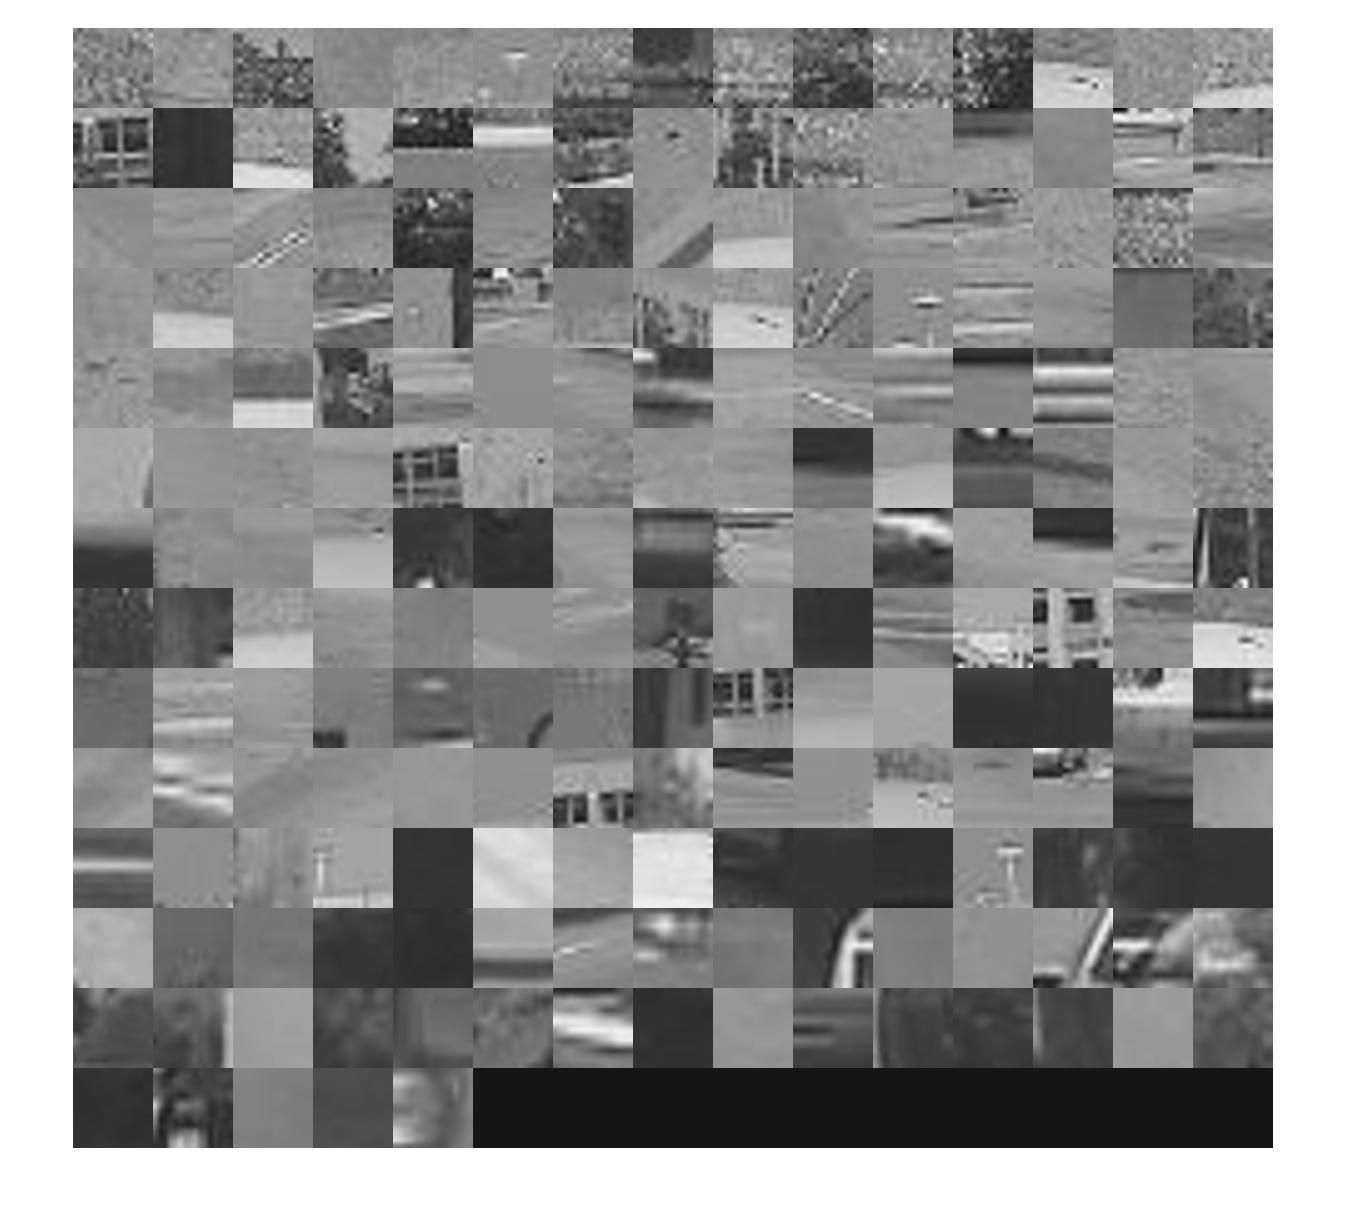
\includegraphics[width=0.9\textwidth]{k200.jpg}
	\caption{Codebook with $k=200$}
	\label{fig1}
\end{figure}
\vspace{5mm}

Note that the black squares on the bottom right do not represent features but are just there to complete the rectangle.

\section{Bag of Words}

Each image feature is assigned to the nearest codebook feature in the function bow histogram using knnsearch for nearest neighbour. The function create bow histograms is used to create the bag of words for all images.



\section{Nearest Neighbours Classifier}

The nearest neighbours classifier is fairly straight forward. Here we compare a selection of features (equal in number to the features in the codebook) to the codebooks with and without cars. if the nearest neighbour is a car we assign the car label, otherwise not. 

\section{Bayesian Classifier}
The bayesian method is more complicated and relies on calculating probabilities instead of one nearest neighbour. In the function computeMeanStd the mean and standart deviation of the features are calculated. The goal is to estimate the probability of a car beeing present given the the histogram of the image. To solve this bayes' theorem was used under the assumption that the features are uncorrelated. The algorithm was implemented into bow recognition bayes as described. Should there be a probability of more than $50\%$ that the image contains a car given the histogram it's classified as such. 

\section{Results}

\subsection{25 Codebook Descriptors}
\vspace{5mm}
\begin{figure}[H]
	\centering
	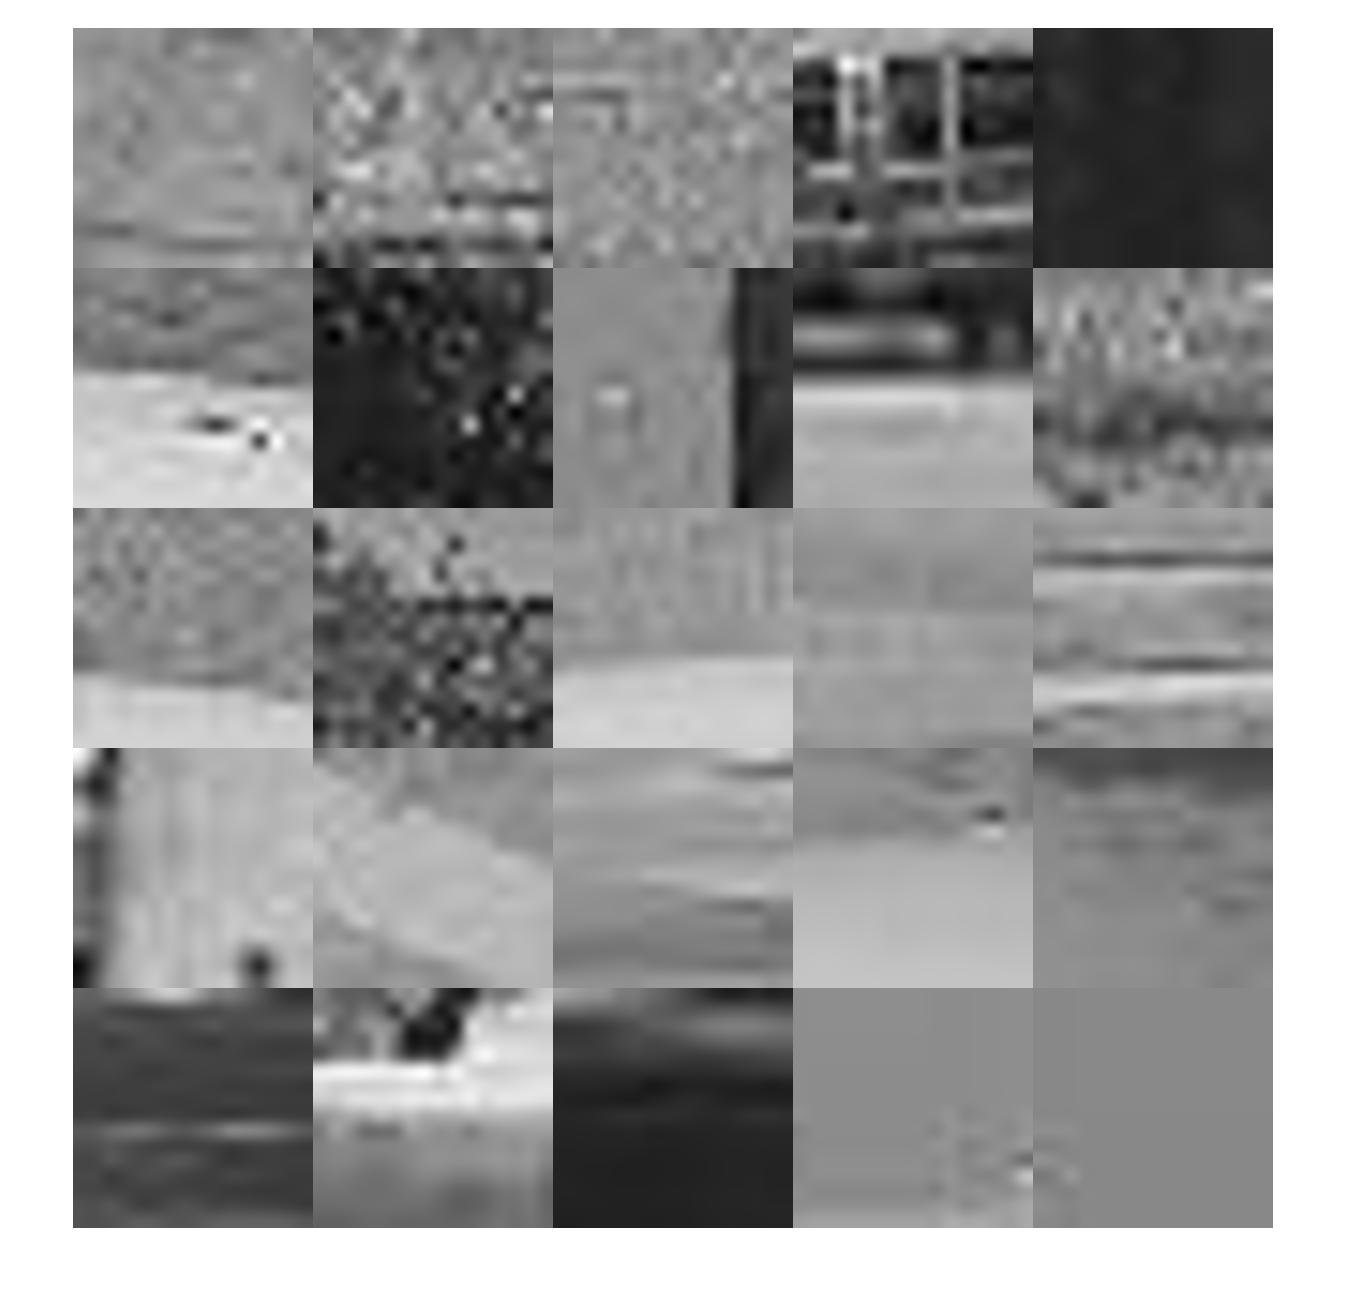
\includegraphics[width=0.9\textwidth]{k25.jpg}
	\caption{Codebook with $k=25$}
	\label{fig1}
\end{figure}
\vspace{5mm}
Nearest neighbour classifier: 
\newline
Percentage of correctly classified images:$90.909\%$
\vspace{5mm}
\newline
Bayesian classifier: 
\newline
Percentage of correctly classified images:$87.879\%$

\subsection{50 Codebook Descriptors}

\vspace{5mm}
\begin{figure}[H]
	\centering
	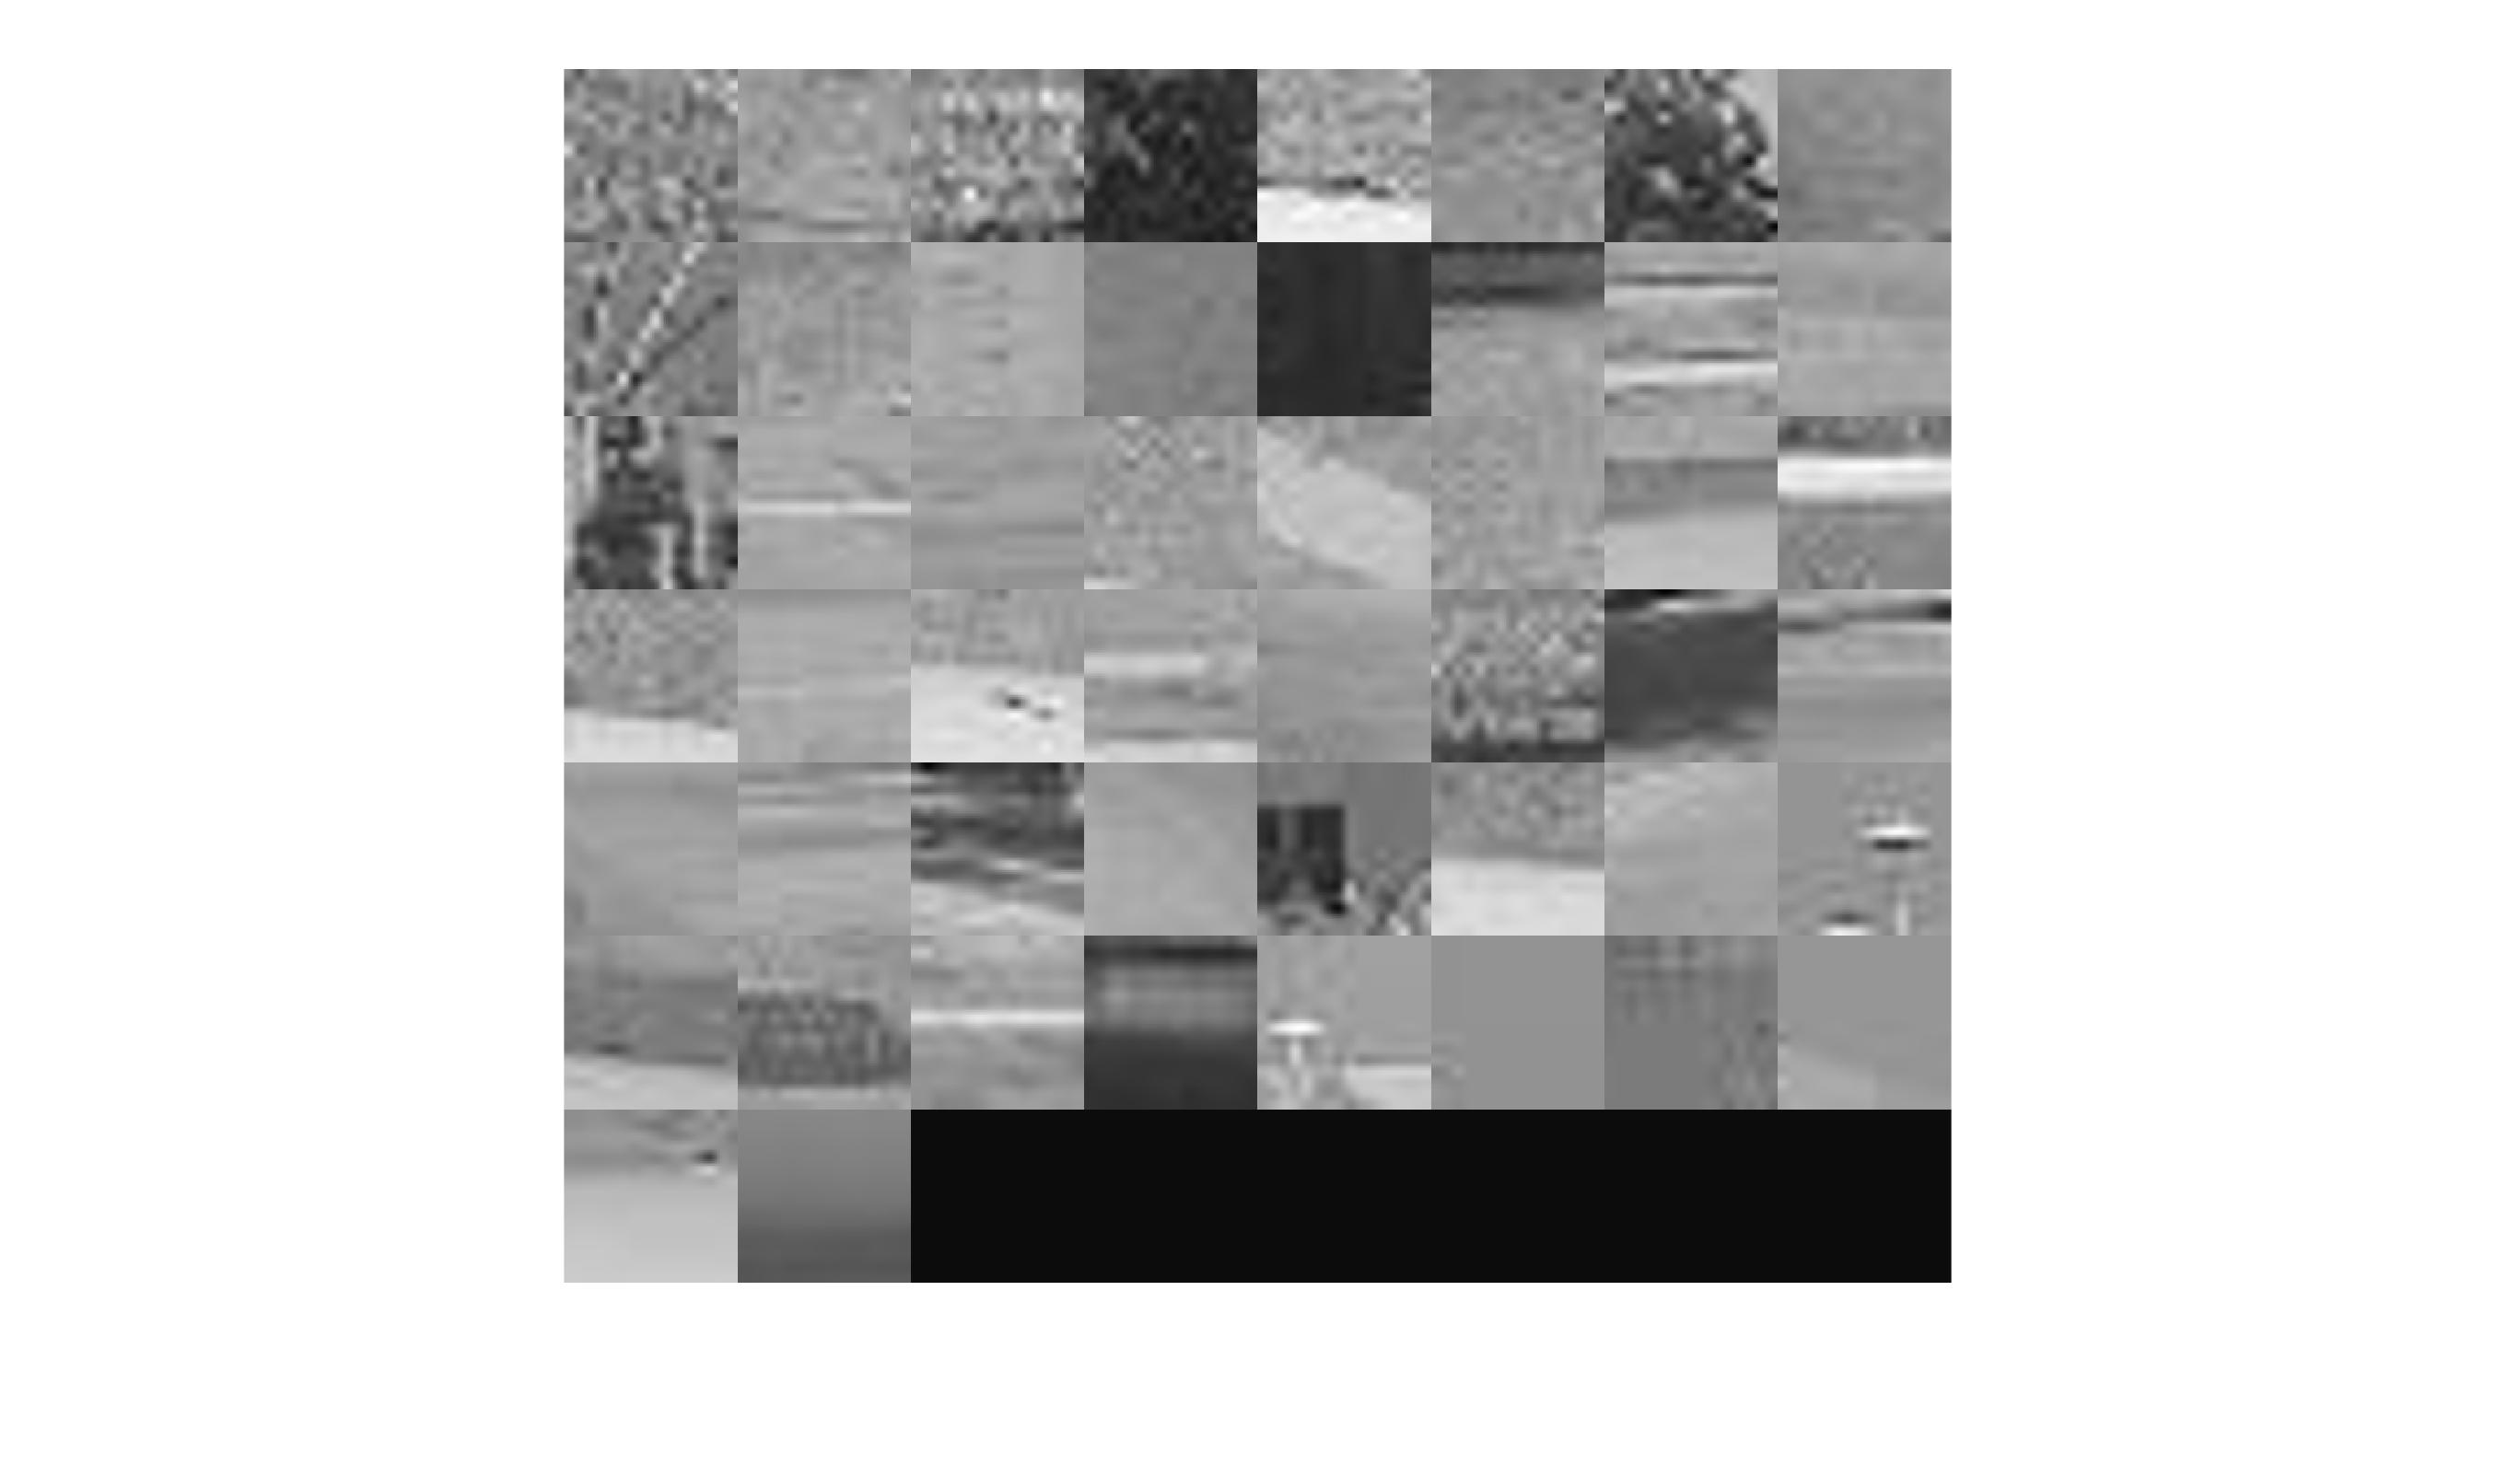
\includegraphics[width=0.9\textwidth]{k50.jpg}
	\caption{Codebook with $k=50$}
	\label{fig1}
\end{figure}
\vspace{5mm}
Nearest neighbour classifier: 
\newline
Percentage of correctly classified images:$94.949\%$
\vspace{5mm}
\newline
Bayesian classifier: 
\newline
Percentage of correctly classified images:$96.97\%$
\subsection{100 Codebook Descriptors}

\vspace{5mm}
\begin{figure}[H]
	\centering
	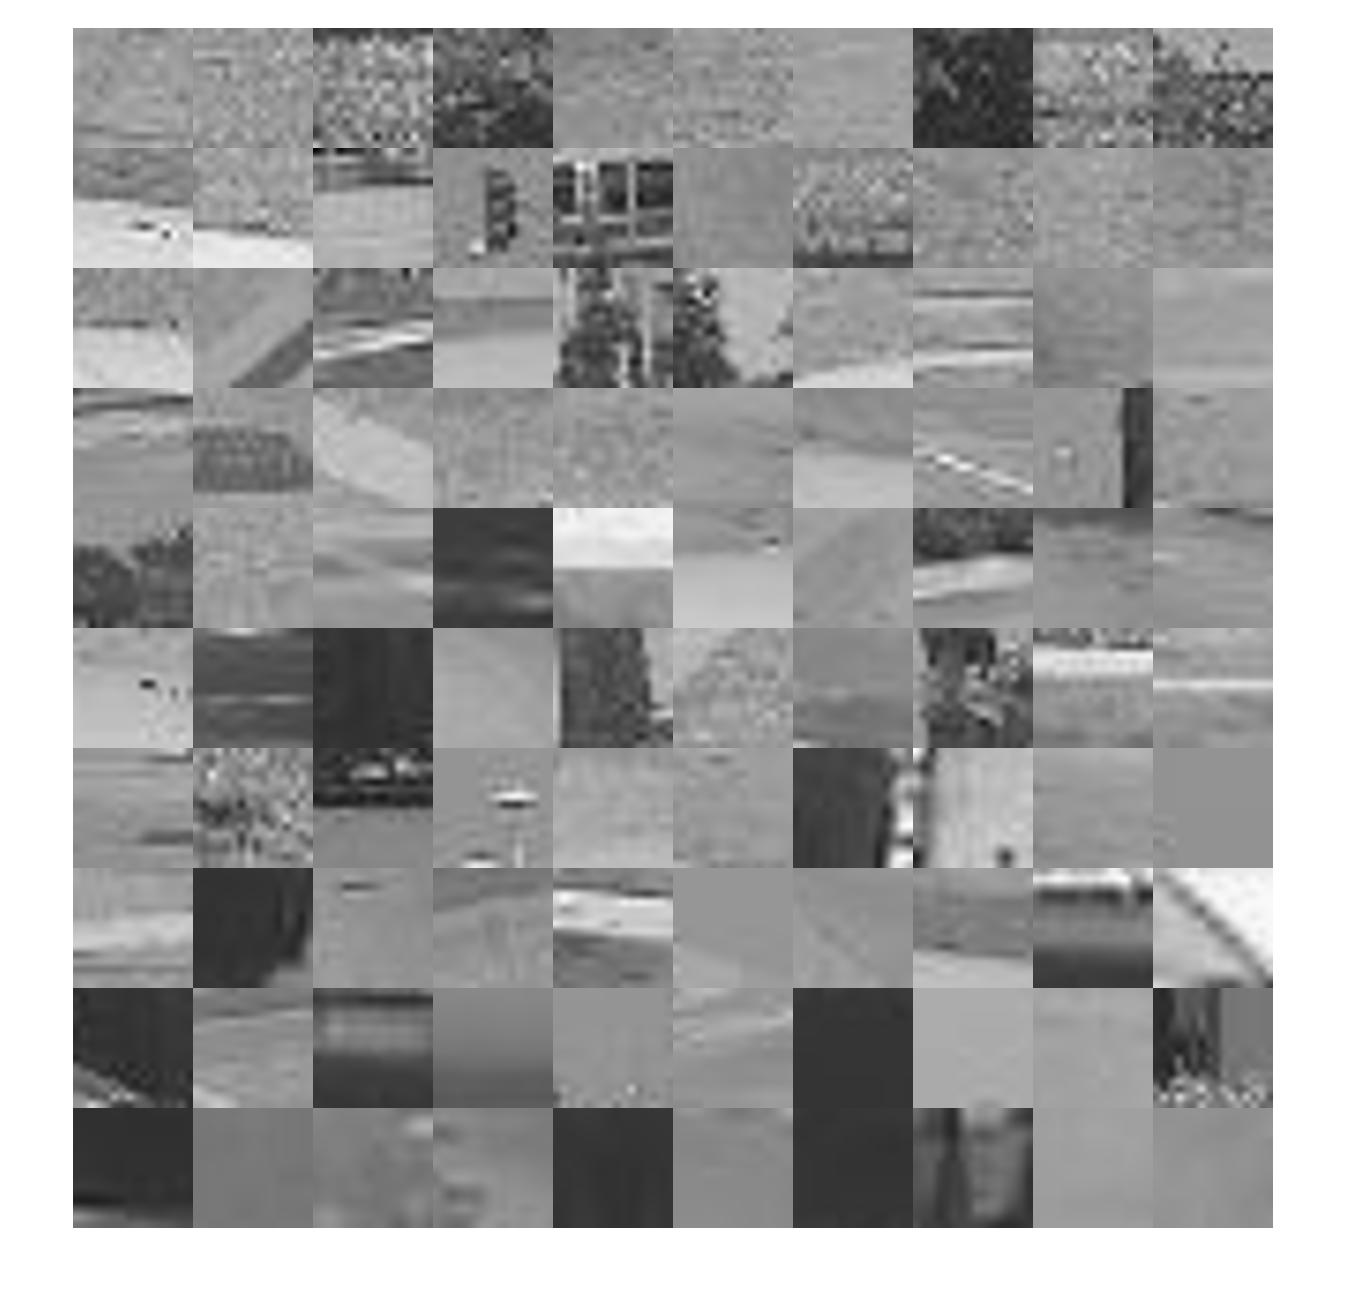
\includegraphics[width=0.9\textwidth]{k100.jpg}
	\caption{Codebook with $k=100$}
	\label{fig1}
\end{figure}
\vspace{5mm}
Nearest neighbour classifier: 
\newline
Percentage of correctly classified images:$93.939\%$
\vspace{5mm}
\newline
Bayesian classifier: 
\newline
Percentage of correctly classified images:$96.978\%$
\subsection{200 Codebook Descriptors}

\vspace{5mm}
\begin{figure}[H]
	\centering
	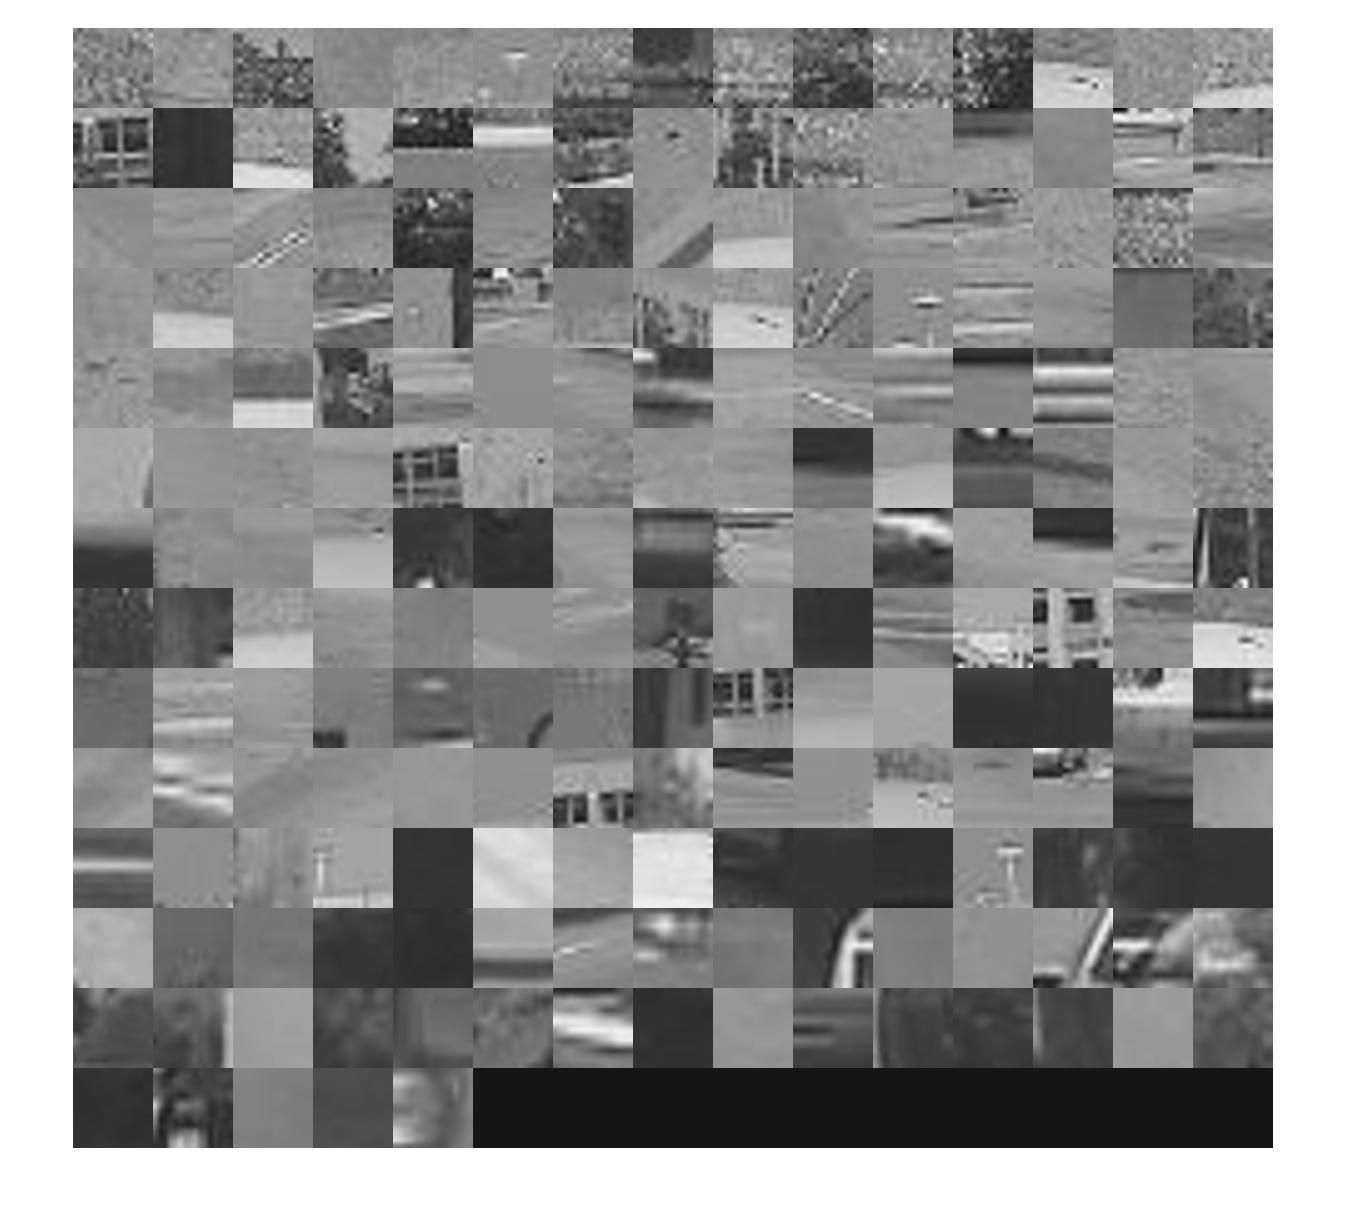
\includegraphics[width=0.9\textwidth]{k200.jpg}
	\caption{Codebook with $k=200$}
	\label{fig1}
\end{figure}
\vspace{5mm}
Nearest neighbour classifier: 
\newline
Percentage of correctly classified images:$91.919\%$
\vspace{5mm}
\newline
Bayesian classifier: 
\newline
Percentage of correctly classified images:$98.99\%$

\subsection{400 Codebook Descriptors}

\vspace{5mm}
\begin{figure}[H]
	\centering
	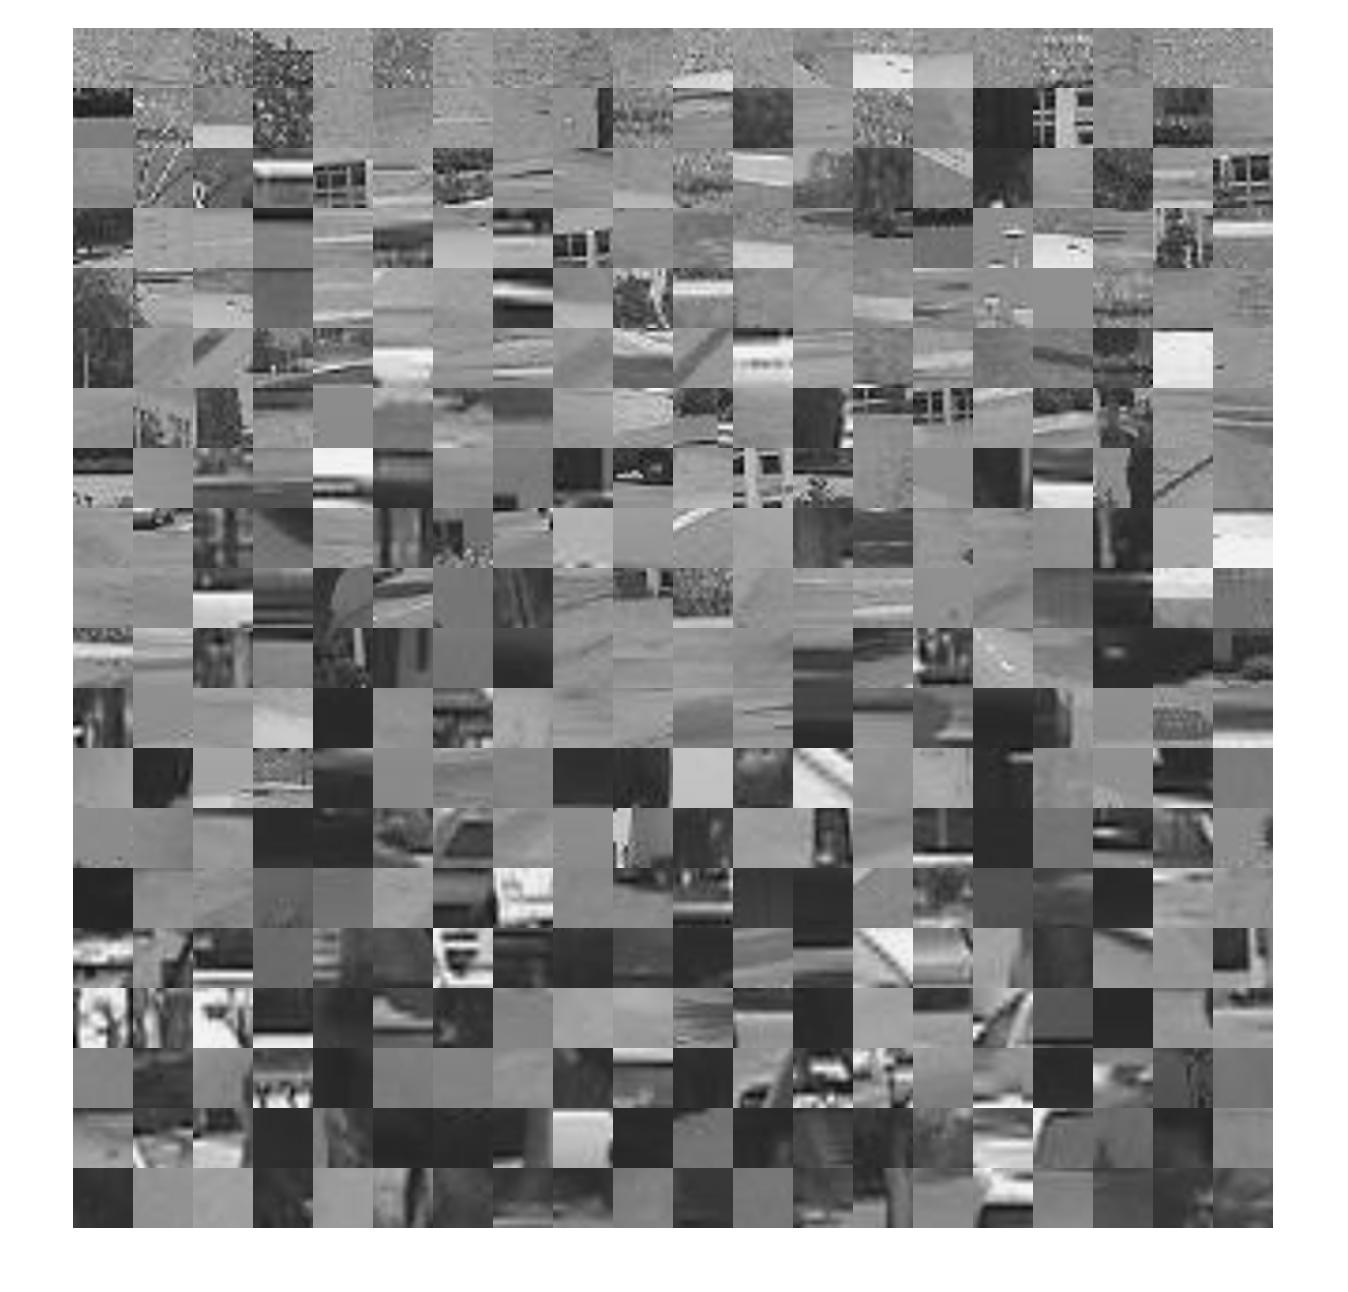
\includegraphics[width=0.9\textwidth]{k400.jpg}
	\caption{Codebook with $k=400$}
	\label{fig1}
\end{figure}
\vspace{5mm}
Nearest neighbour classifier: 
\newline
Percentage of correctly classified images:$94.949\%$
\vspace{5mm}
\newline
Bayesian classifier: 
\newline
Percentage of correctly classified images:$100\%$

\section{Discussion}

\vspace{5mm}
\begin{figure}[H]
	\centering
	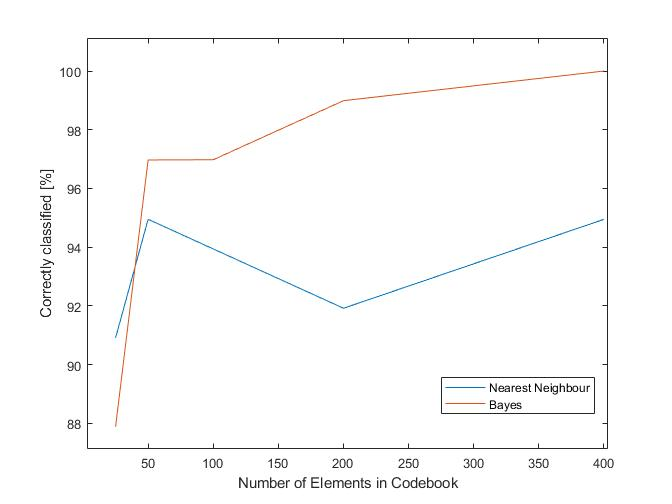
\includegraphics[width=0.9\textwidth]{plot.jpg}
	\caption{Performance of the two algorithms}
	\label{fig1}
\end{figure}
\vspace{5mm}
As can be seen the Bayesian classifier outruns the nearest neighbour classifiers for all k except of at 25. This makes sense, since we feed our "model" with some prior belief about the world. As expected, the accuracy of the Bayesian classifier increases steadily which increasing Codebook size, this makes sense, since we get a more accurate description of the training data. Strangely this seems not to be strictly the case for the nearest neighbour. 
\newline
Since theese measures vary a bit from run to run more testing would be needed for a statistically relevant sample. 
\end{document}

